
\section{Comparison with Python Adaptation}

In this section, we compare the results presented in the paper \cite{pyle2019} with the MATLAB implementation by the authors and our Python adaptation. The original scripts, although not available online, are readily available on request. We present our adaptation of this model in the open source framework Python, which has been built based on the paper and the MATLAB scripts provided by the authors. In contrast to the original scripts, it is modular and is easily modifiable with external json descriptor files. We compare the results presented in the paper, with simulations of the MATLAB scripts, provided by the authors, and also with our adaptation in Python  \footnote{In Figures~\ref{Fig:Comparison_Task1}-~\ref{Fig:Comparison_Task3}, the results presented in the paper have been reused in the column titled "original".}.\\ 

To validate our Python adaptation, we test the three algorithms on three tasks by simulating them using both the original scripts and our Python adaptation. For each algorithm-task combination, we produce ten simulations with arbitrary seeds initialising the random generator and one additional simulation using the default seed of MATLAB (equivalent to seed 5489 of the numpy random generator). Except for the default seed, the ten arbitrary seeds are different for the Python and MATLAB simulations, and for each algorithm-task combination. Both MATLAB and numpy use the Mersenne Twister pseudo-random number generator \cite{matsumoto1998}. To evaluate the performance of the algorithm, the authors plot the ``distance from target", i.e. the square root of the low pass filtered version of the mean squared error, over the progression of the simulation. In order to categorise the model performance as satisfactory or unsatisfactory, we further compute a \textbf{deviation metric} by calculating the mean ``distance from target" over the testing phase. If this deviation metric is below the threshold of 0.5 (set by visual inspection), the model is said to have satisfactorily learnt and produced the target output.



\subsection{Task 1}

Here, we compare the simulations of the original scripts and our adaptation for Task 1, using FORCE, RMHL and SUPERTREX, with the results presented in the article. Task 1 is designed to test the performance of these three algorithms when generating a known target output. The objective of this task is to produce a time-series of 2-D coordinates required to traverse a target trajectory, in this case, the parameterized curve of a butterfly. The model is trained to generate an output which closely matches the target function. \\ 

The article claims that:
\begin{itemize}
\item under the FORCE framework, the target time-series is learned accurately and is maintained in a stable manner during the testing phase (Figure~\ref{Fig:compTask1FORCE}).
\item under the RMHL framework, the target time-series is generated accurately during the training phase, however is not maintained perfectly during the testing phase (Figure~\ref{Fig:compTask1RMHL}).
\item under the SUPERTREX framework, the target time-series is learned accurately and is also maintained in a stable manner during testing phase, albeit not as well as FORCE (Figure~\ref{Fig:compTask1ST}).
\end{itemize}

We validate these observations with the MATLAB scripts provided by the authors as well as with our Python adaptation. To do so, we run the simulations with the default seed and repeat it ten times with different (arbitrarily chosen) seeds initialising the random number generator.  


We observe that:
\begin{itemize}
\item under the FORCE framework, the target time-series is learned accurately and is maintained in a stable manner during the testing phase, as claimed. The mean deviation over eleven simulations, for both the original scripts ($0.003\pm0.002$; n=11) and the Python adaptation ($0.004\pm0.003$; n=11) is much lower than the threshold of 0.5 (Figure~\ref{Fig:compTask1FORCE},~\ref{Fig:compTask1FORCE_MSE}).
\item under the RMHL framework, the target time-series is generated accurately during the training phase, however is not maintained perfectly during the testing phase, as claimed. The mean deviation, for both the original scripts ($0.168\pm0.038$; n=11) and the Python adaptation ($0.182\pm0.046$; n=11), is higher than that with FORCE (Figure~\ref{Fig:compTask1RMHL},~\ref{Fig:compTask1RMHL_MSE}).
\item under the SUPERTREX framework, the target time-series is learned accurately and is also maintained in a stable manner during testing phase, albeit not as well as FORCE, as claimed. The mean deviation, for both the original scripts ($0.006\pm0.003$; n=11) and the Python adaptation ($0.006\pm0.003$; n=11), is much better than that for RMHL, but slightly worse than with FORCE (Figure~\ref{Fig:compTask1ST}, ~\ref{Fig:compTask1ST_MSE}).

\end{itemize}

Both the original scripts and the Python adaptation are able to successfully closely reproduce the results presented in the paper for Task 1 (Figure~\ref{Fig:Comparison_Task1},\ref{Fig:Comparison_Task1_MSE}; Table~\ref{Table:deviation_tasks},~\ref{Table:deviation_prop_tasks}).

\begin{figure}

    \centering
    \textbf{MATLAB}\hspace{8em}
    \textbf{Original}\hspace{8em}
    \textbf{Python}
    
    \begin{subfigure}{\textwidth}
        \centering
        
        \textbf{\rotatebox[origin=c]{90}{FORCE}}\begin{subfigure}{\textwidth}
        \centering
    
        % 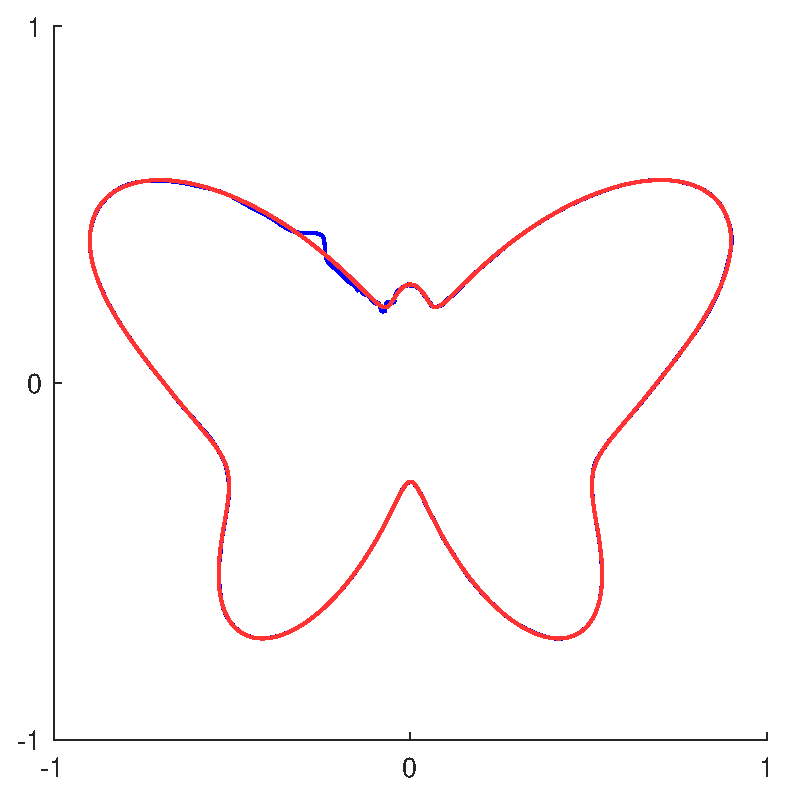
\includegraphics[trim=1.5cm 3cm 1.5cm 3cm, clip=true, height=.2\linewidth]{Figures/Fig_T1/MATLAB/FORCE_T1_Trajectory_axis}
        \includegraphics[trim=1.5cm 2cm 1.5cm 2cm, clip=true,height=.1\textheight]{Figures/Fig_T1/MATLAB/FORCE_T1_Trajectory_noaxis}
        \hspace{3em}
        \includegraphics[height=.08\textheight]{Figures/Fig_T1/Orig/FORCE_T1_Trajectory}
        \hspace{3em}
        \includegraphics[trim=1.5cm 2cm 1.5cm 2cm, clip=true,height=.1\textheight]{Figures/Fig_T1/Python/FORCE_T1_Trajectory_noaxis}

        \end{subfigure}
         
         
        \textbf{\rotatebox[origin=c]{90}{x(t)}}\begin{subfigure}{\textwidth}
        \centering
        
        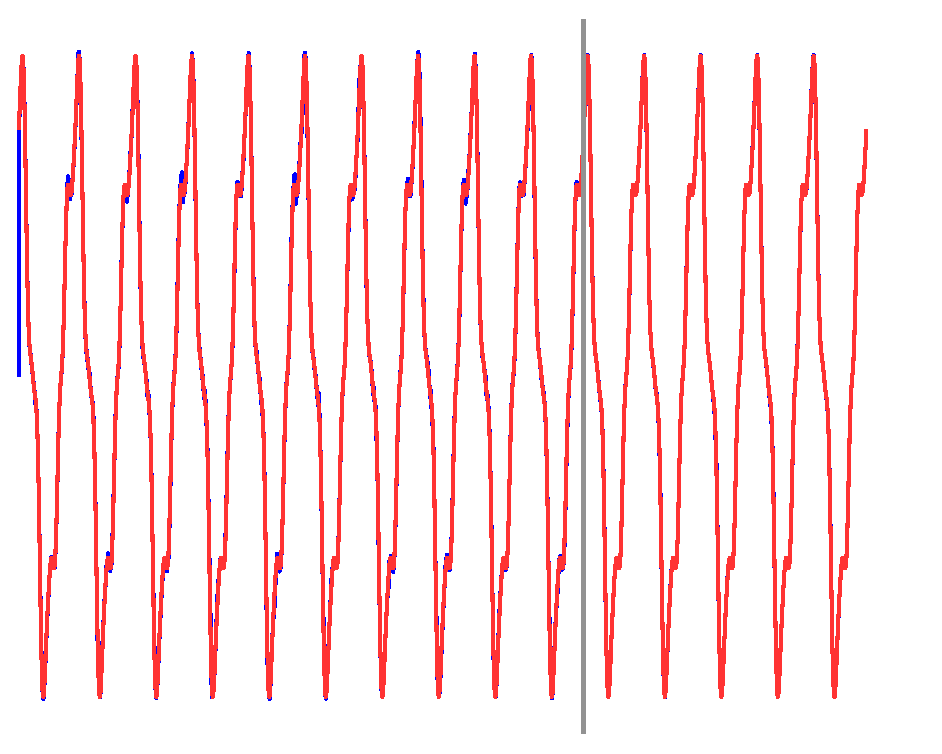
\includegraphics[height=0.08\linewidth,width=.45\linewidth]{Figures/Fig_T1/MATLAB/FORCE_T1_CoordinateX}
        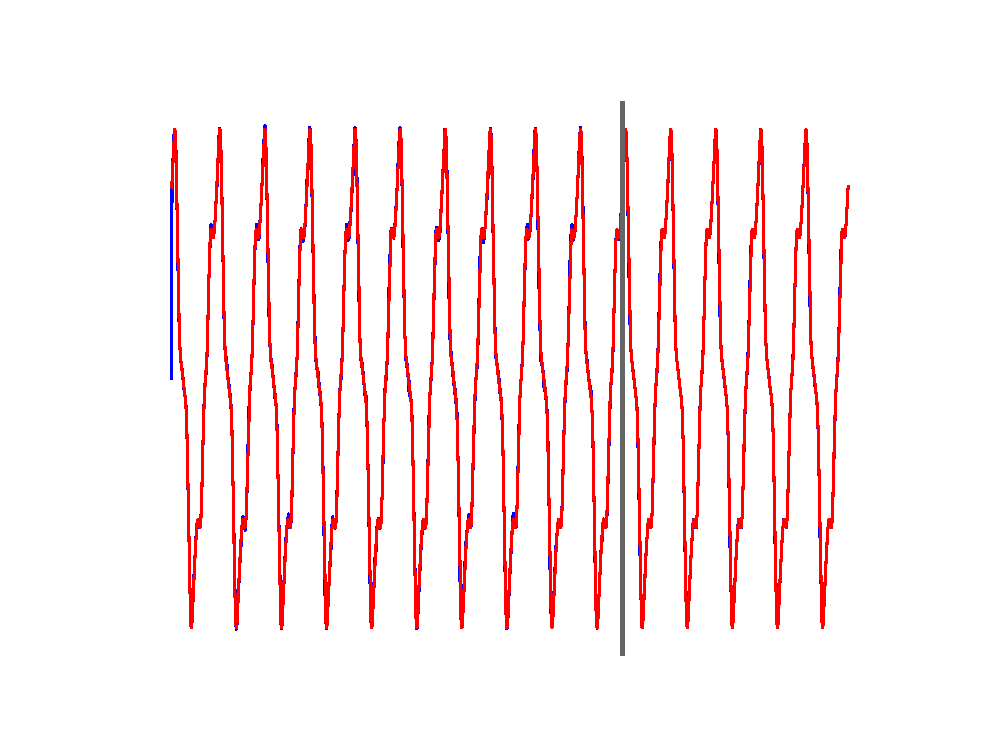
\includegraphics[trim=2cm 1cm 2cm 1cm, clip=true,height=0.08\linewidth,width=.45\linewidth]{Figures/Fig_T1/Python/FORCE_T1_CoordinateX}
        
        \end{subfigure}
        
        
        \textbf{\rotatebox[origin=c]{90}{y(t)}}\begin{subfigure}{\textwidth}
        \centering
        
        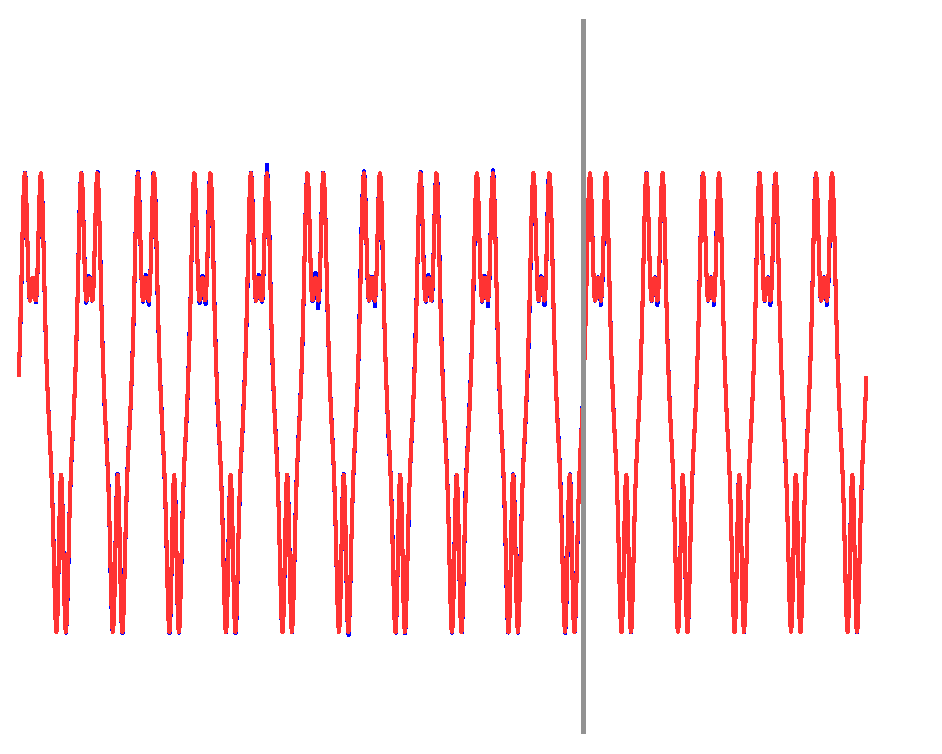
\includegraphics[height=0.08\linewidth,width=.45\linewidth]{Figures/Fig_T1/MATLAB/FORCE_T1_CoordinateY}
        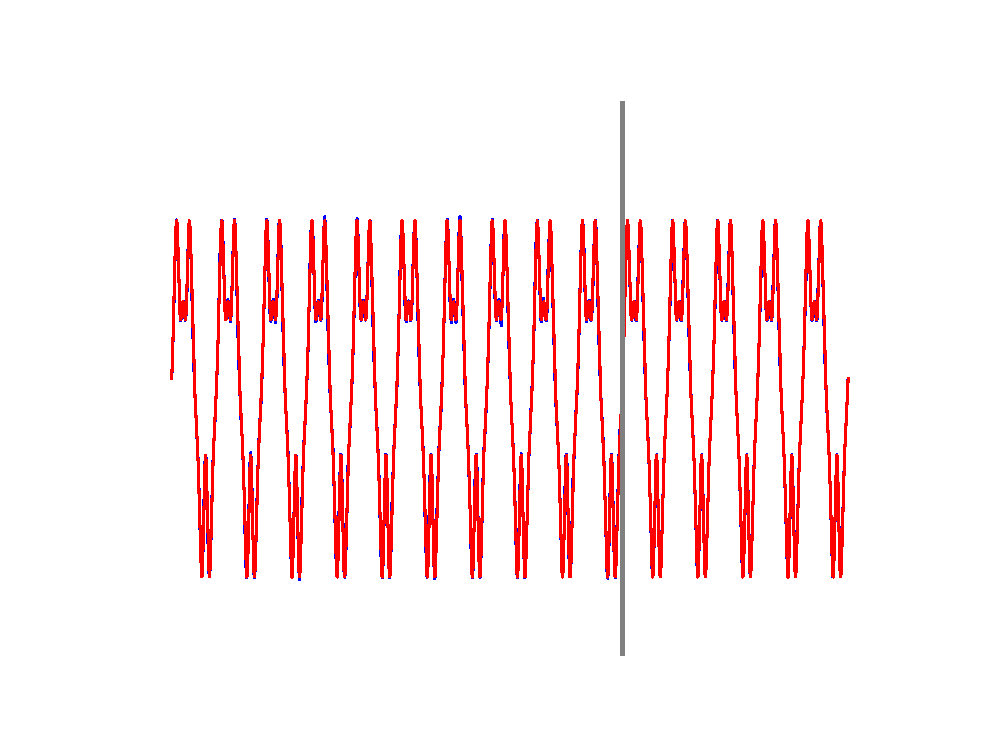
\includegraphics[trim=2cm 1cm 2cm 1cm, clip=true,height=0.08\linewidth,width=.45\linewidth]{Figures/Fig_T1/Python/FORCE_T1_CoordinateY}
        
        \end{subfigure}
        

    \caption{Results for Task 1 with the FORCE algorithm. The target time‐series is learned accurately during the training phase and is maintained in a stable manner during the testing phase, in both implementations, as presented in \cite{pyle2019}.}
    \label{Fig:compTask1FORCE}
    \end{subfigure}

    \begin{subfigure}{\textwidth}
        \centering
        
        \textbf{\rotatebox[origin=c]{90}{RMHL}}\begin{subfigure}{\textwidth}
        \centering
        
        
\includegraphics[trim=3cm 4cm 3cm 4cm, clip=true,height=.1\textheight]{Figures/Fig_T1/MATLAB/RHML_T1_Trajectory}
        \hspace{4em}
        
\includegraphics[height=.08\textheight]{Figures/Fig_T1/Orig/RMHL_T1_Trajectory}
        \hspace{4em}
        
\includegraphics[trim=6cm 4.5cm 6cm 4.5cm, clip=true,height=.1\textheight]{Figures/Fig_T1/Python/RHML_T1_Trajectory}
        
        \end{subfigure}
         
        
        
        \textbf{\rotatebox[origin=c]{90}{x(t)}}\begin{subfigure}{\textwidth}
        \centering
        
        \includegraphics[height=0.08\linewidth,width=.45\linewidth]{Figures/Fig_T1/MATLAB/RHML_T1_CoordinateX}
        \includegraphics[trim=2cm 1cm 2cm 1cm, clip=true,height=0.08\linewidth,width=.45\linewidth]{Figures/Fig_T1/Python/RHML_T1_CoordinateX}
        
        \end{subfigure}
         
        
        
        \textbf{\rotatebox[origin=c]{90}{y(t)}}\begin{subfigure}{\textwidth}
        \centering
        
        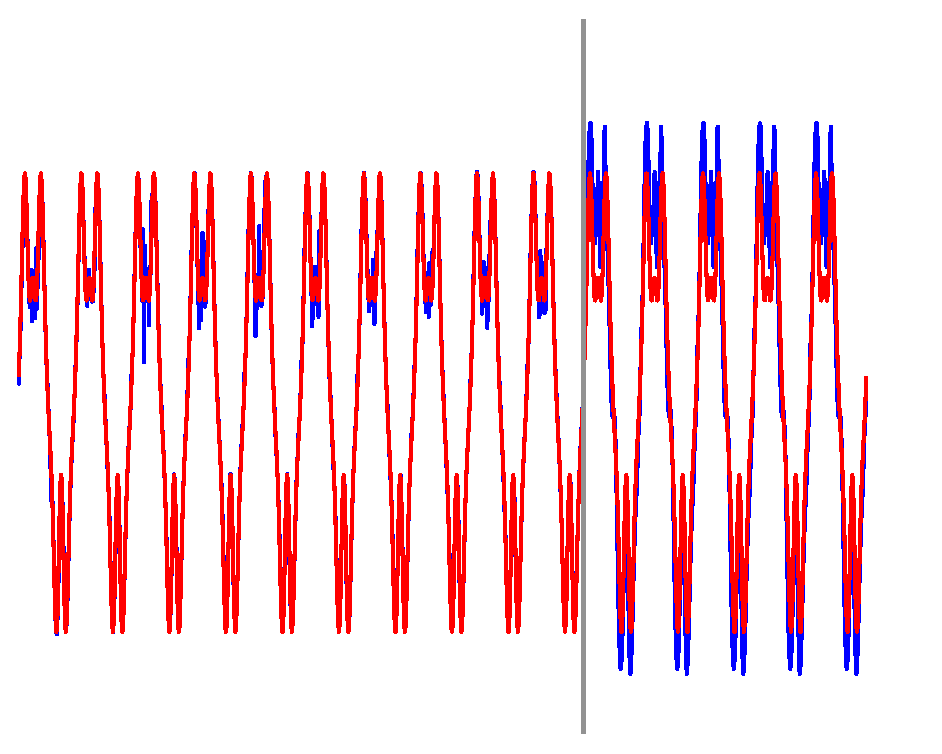
\includegraphics[height=0.08\linewidth,width=.45\linewidth]{Figures/Fig_T1/MATLAB/RHML_T1_CoordinateY}
        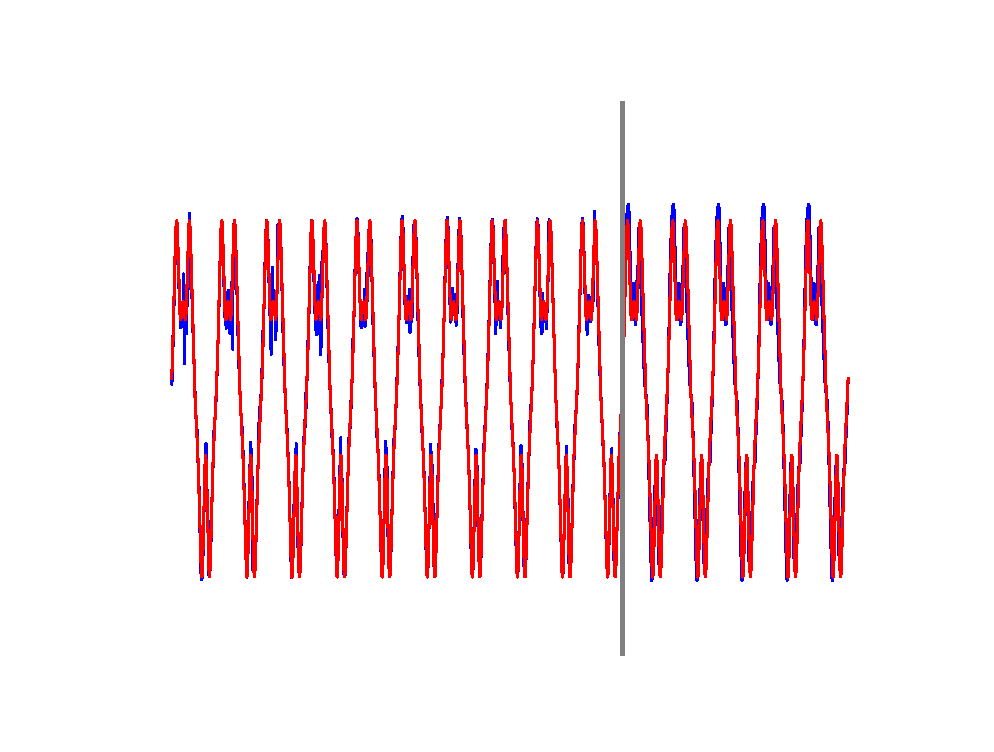
\includegraphics[trim=2cm 1cm 2cm 1cm, clip=true,height=0.08\linewidth,width=.45\linewidth]{Figures/Fig_T1/Python/RHML_T1_CoordinateY}
        
        \end{subfigure}
        
    \caption{Results for Task 1 with the RMHL algorithm. The target time‐series is learned accurately during the training phase, though not maintained perfectly during the testing phase, in both implementations, as presented in \cite{pyle2019}.}
    \label{Fig:compTask1RMHL}
    \end{subfigure}
    
    \begin{subfigure}{\textwidth}
        \centering
        
        \textbf{\rotatebox[origin=c]{90}{SUPERTREX}}\begin{subfigure}{\textwidth}
        \centering
        
        
\includegraphics[trim=3cm 4cm 3cm 4cm, clip=true,height=.1\textheight]{Figures/Fig_T1/MATLAB/ST_T1_Trajectory.eps}
        \hspace{4em}
        
\includegraphics[height=.08\textheight]{Figures/Fig_T1/Orig/ST_T1_Trajectory.png}
        \hspace{4em}
        
\includegraphics[trim=6cm 4.5cm 6cm 4.5cm,clip=true,height=.1\textheight]{Figures/Fig_T1/Python/ST_T1_Trajectory.eps}
        
        \end{subfigure}
         
        
        
        \textbf{\rotatebox[origin=c]{90}{x(t)}}\begin{subfigure}{\textwidth}
        \centering
        
        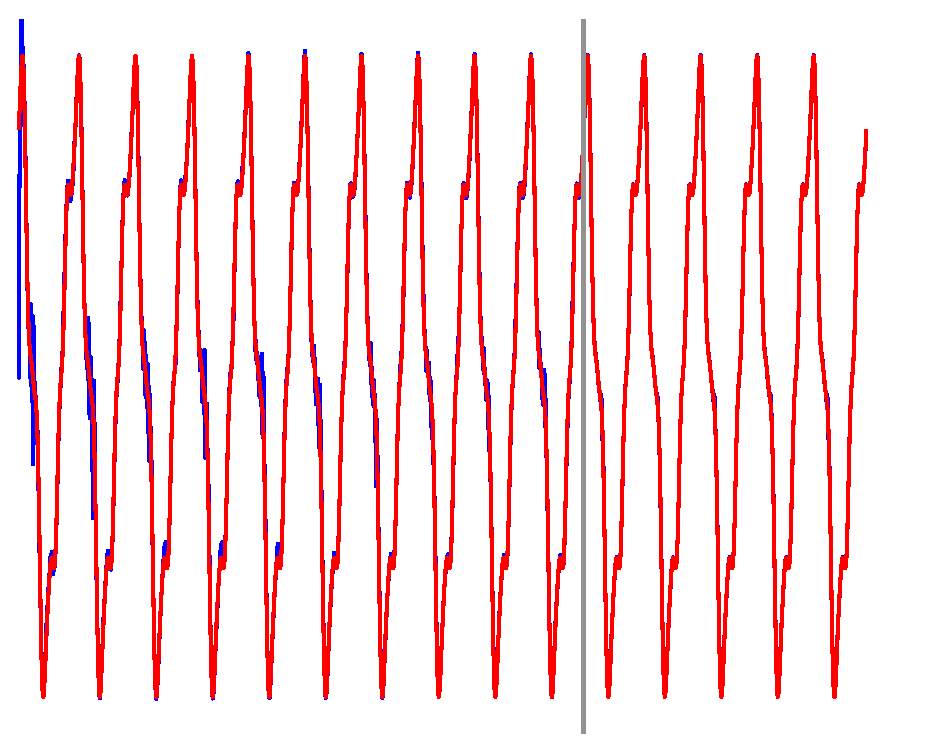
\includegraphics[height=0.08\linewidth,width=.4\linewidth]{Figures/Fig_T1/MATLAB/ST_T1_CoordinateX}
        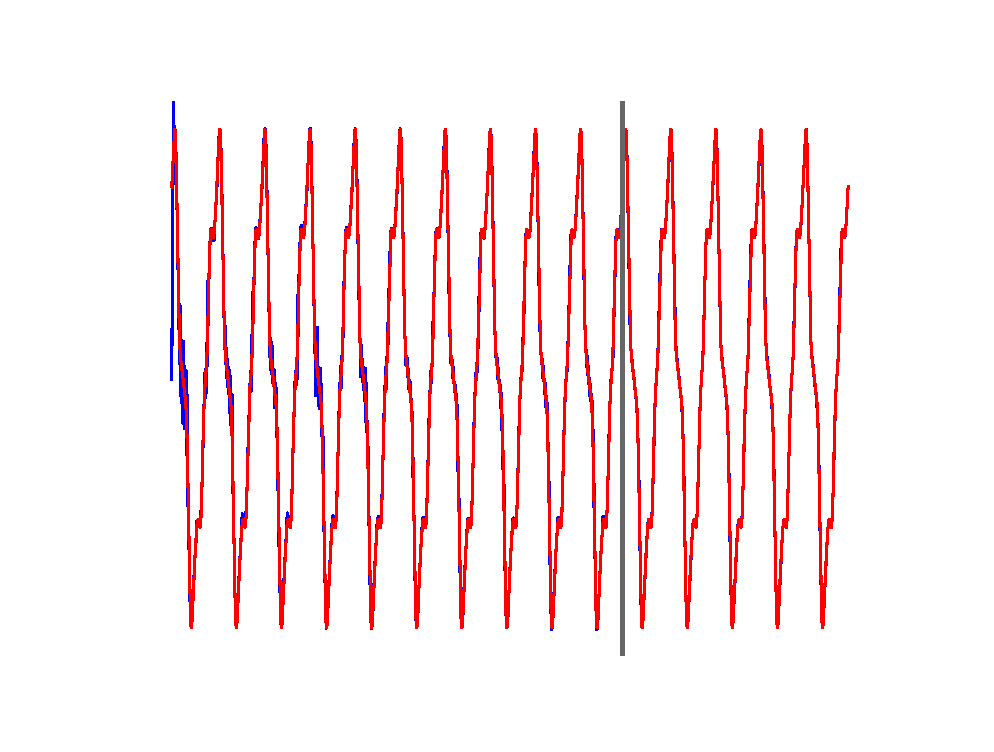
\includegraphics[trim=2cm 1cm 2cm 1cm, clip=true,height=0.08\linewidth,width=.45\linewidth]{Figures/Fig_T1/Python/ST_T1_CoordinateX}
        
        \end{subfigure}
         
        
        
        \textbf{\rotatebox[origin=c]{90}{y(t)}}\begin{subfigure}{\textwidth}
        \centering
        
        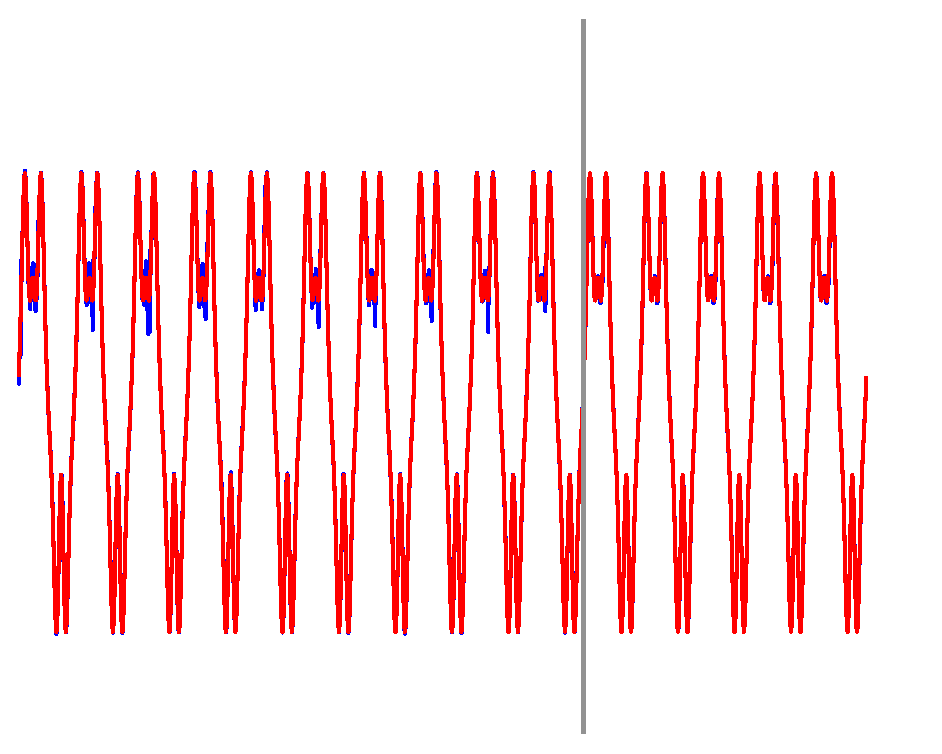
\includegraphics[height=0.08\linewidth,width=.4\linewidth]{Figures/Fig_T1/MATLAB/ST_T1_CoordinateY}
        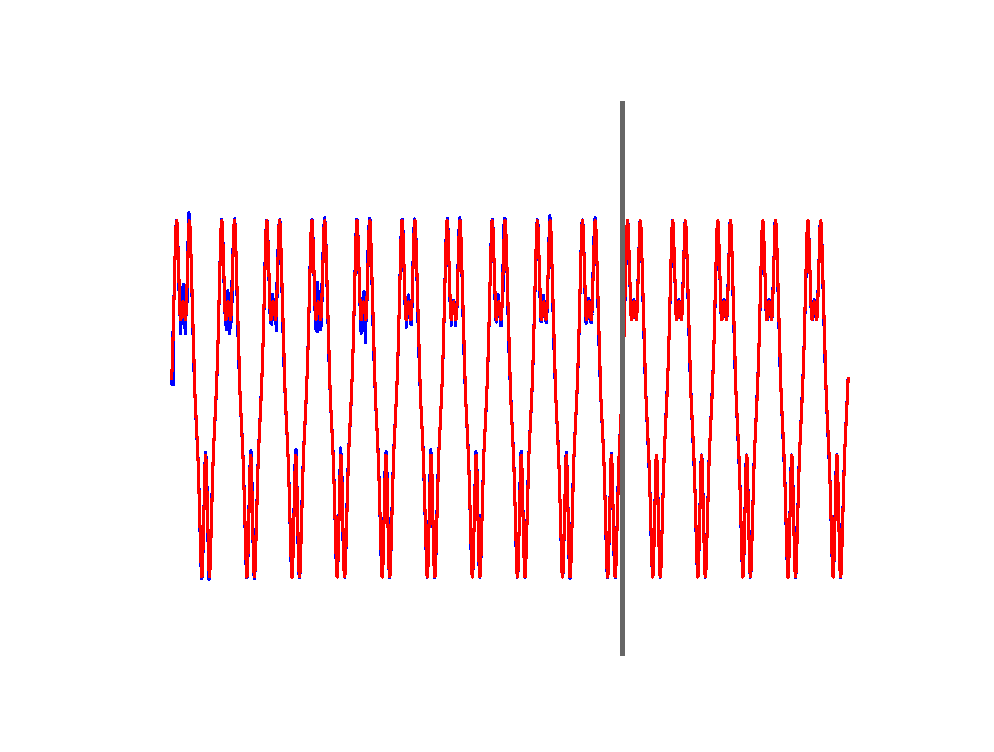
\includegraphics[trim=2cm 1cm 2cm 1cm, clip=true,height=0.08\linewidth,width=.45\linewidth]{Figures/Fig_T1/Python/ST_T1_CoordinateY}
        
        \end{subfigure}
        
        
        
        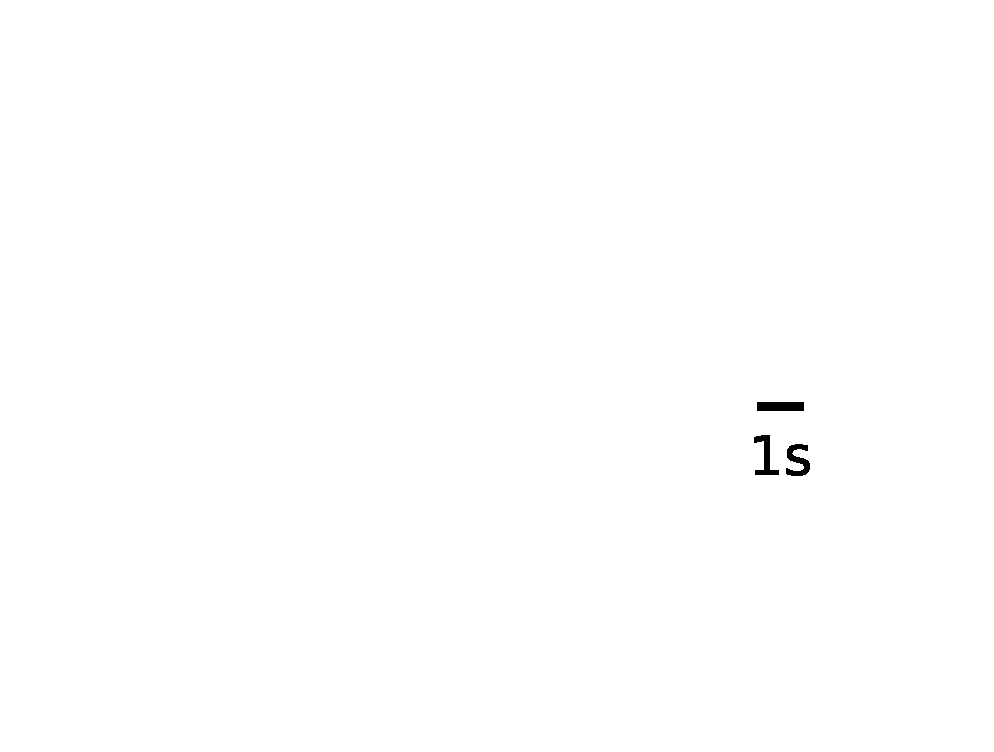
\includegraphics[trim=2cm 6cm 2cm 6cm, clip=true,height=0.05\linewidth,width=.4\linewidth]{Figures/Fig_T1/Python/ST_T1_Scale.eps}
        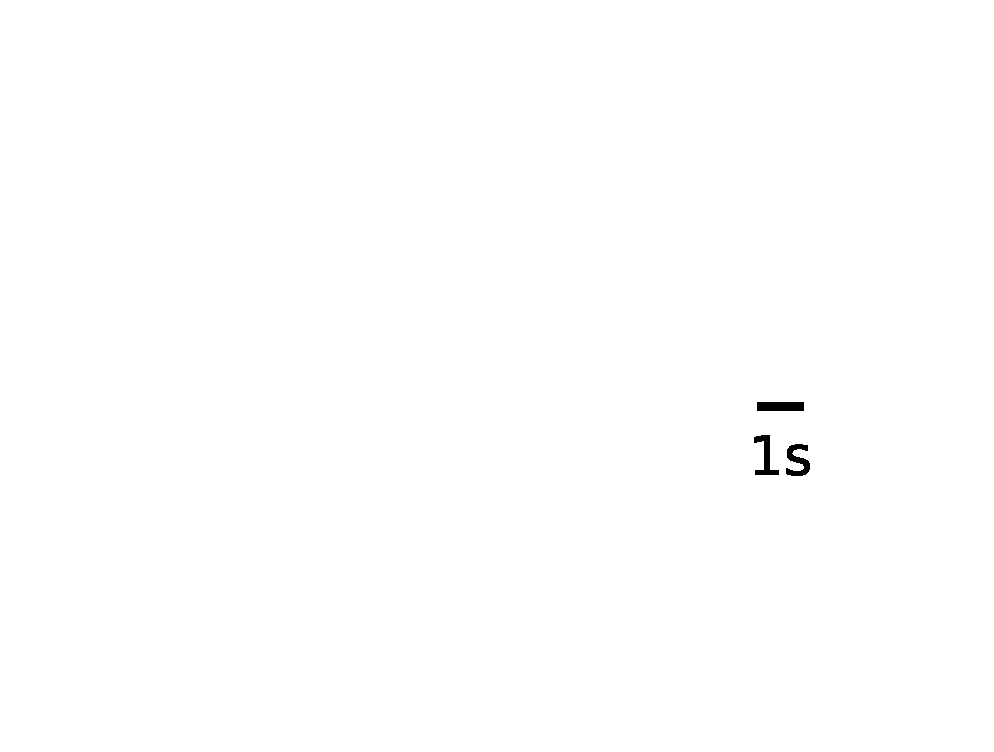
\includegraphics[trim=2cm 4cm 2cm 6cm, clip=true,height=0.05\linewidth,width=.45\linewidth]{Figures/Fig_T1/Python/ST_T1_Scale.eps}
        

    \caption{Results for Task 1 with the SUPERTREX algorithm. The target time‐series is learned accurately during the training phase, and is also maintained in a stable manner during testing phase, albeit not as well as FORCE, in both implementations, as presented in \cite{pyle2019}.}
    \label{Fig:compTask1ST}
    
    \end{subfigure}


\caption{Comparison of the performances of the MATLAB scripts (left column) and the Python adaptation (right column) with the results presented in the original article (center column), for the three learning algorithms on Task 1 \cite{pyle2019}. All simulations shown here use the MATLAB default (5489) as the seed for the random number generator. In each subfigure, the top row shows the target trajectory (red) with the trajectory generated by the model (blue) throughout the test phase. The second row shows the time-series (blue) generated by the model (x and y coordinates, in this case) along with the target time-series (red). The grey vertical line marks the separation of the training and testing phase.}
\label{Fig:Comparison_Task1}

\end{figure}


\begin{figure}

    \centering
    \textbf{MATLAB}\hspace{8em}
    \textbf{Original}\hspace{8em}
    \textbf{Python}
    
    \begin{subfigure}{\textwidth}
        \centering
        
        \textbf{\rotatebox[origin=c]{90}{FORCE}}\begin{subfigure}{\textwidth}
        \centering
    
        \includegraphics[trim=1.5cm 2cm 1.5cm 2cm, clip=true,height=.1\textheight]{Figures/Fig_T1/MATLAB/FORCE_T1_Trajectory_noaxis}
        \hspace{3em}
        \includegraphics[height=.08\textheight]{Figures/Fig_T1/Orig/FORCE_T1_Trajectory}
        \hspace{3em}
        \includegraphics[trim=1.5cm 2cm 1.5cm 2cm, clip=true,height=.1\textheight]{Figures/Fig_T1/Python/FORCE_T1_Trajectory_noaxis}

        \end{subfigure}
         
         
        \textbf{\rotatebox[origin=c]{90}{MSE}}\begin{subfigure}{\textwidth}
        \centering
        
        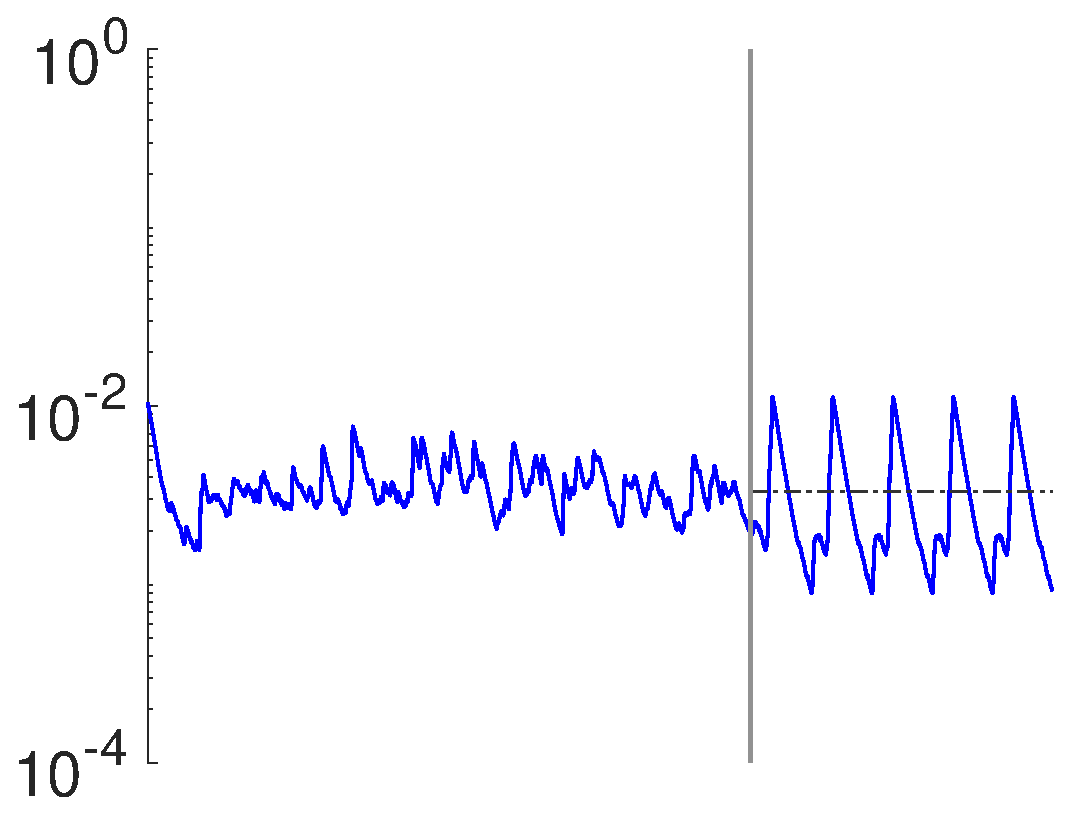
\includegraphics[height=0.12\linewidth,width=.45\linewidth]{Figures/Fig_T1/MATLAB/FORCE_T1_MSE.eps}
        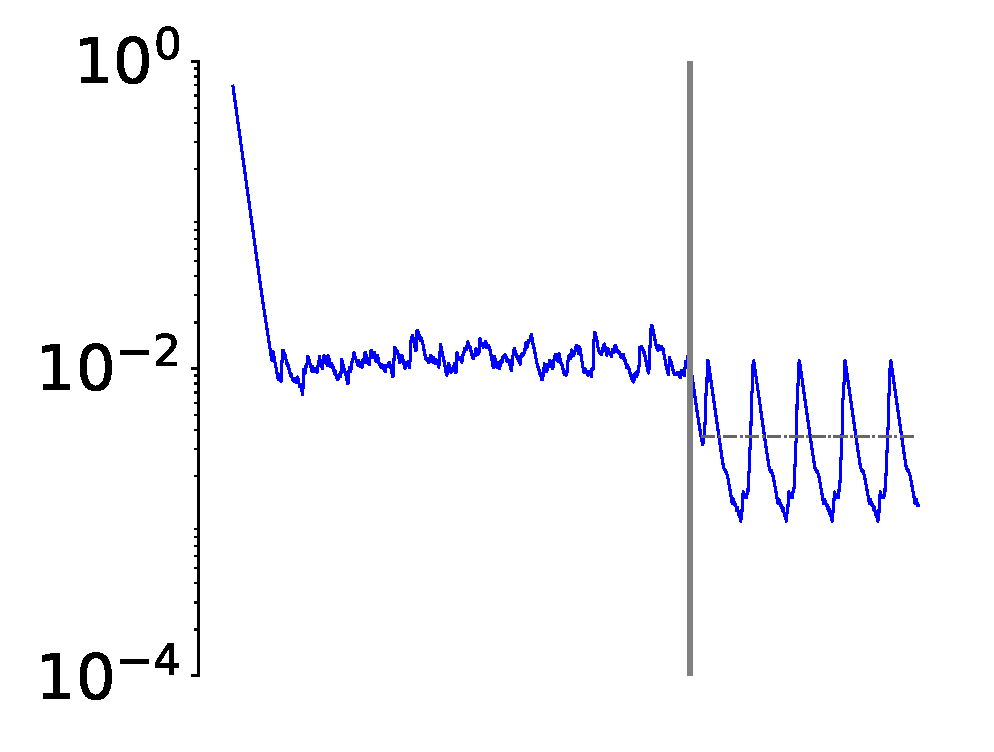
\includegraphics[height=0.12\linewidth,width=.45\linewidth]{Figures/Fig_T1/Python/FORCE_T1_MSE.eps}
        
        \end{subfigure}
        
        
        \textbf{\rotatebox[origin=c]{90}{||W||}}\begin{subfigure}{\textwidth}
        \centering
        
        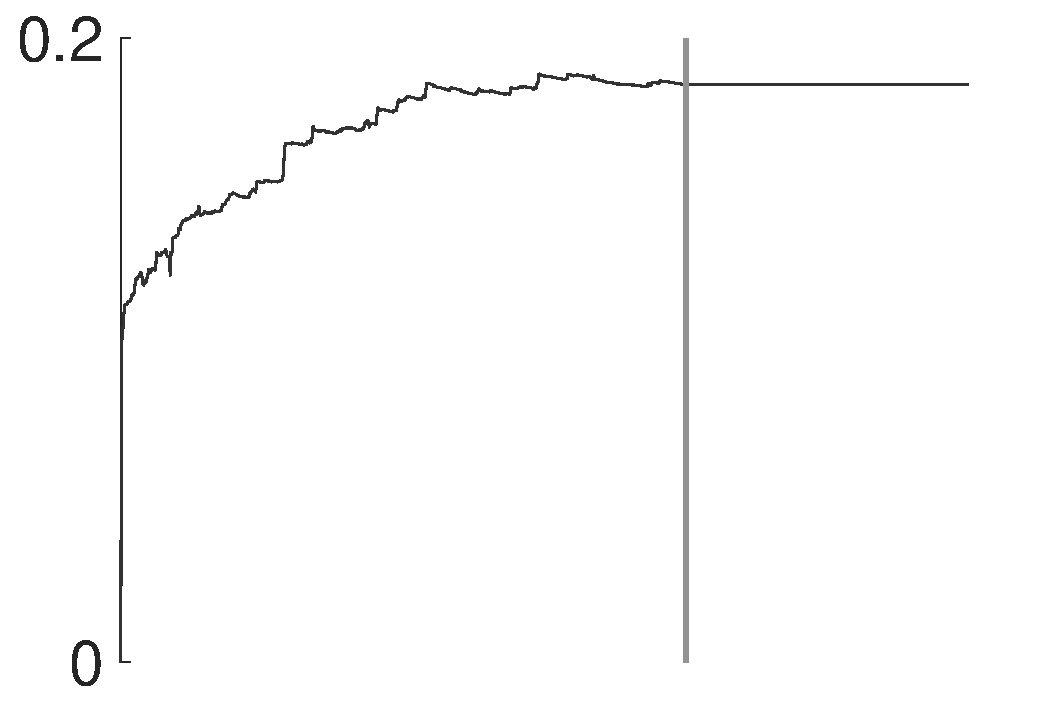
\includegraphics[trim=0cm 0cm 1cm 0cm, clip=true,height=0.12\linewidth,width=.45\linewidth]{Figures/Fig_T1/MATLAB/FORCE_T1_W_norm.eps}
        \hspace{.3em}
        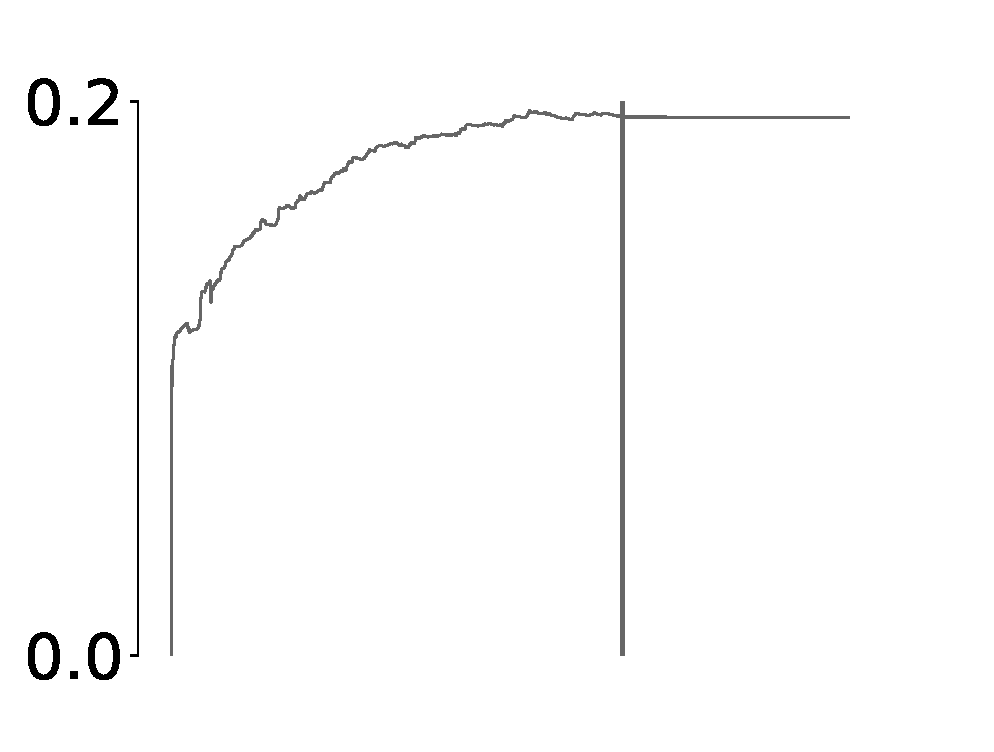
\includegraphics[trim=0cm 0cm 1cm 0cm, clip=true,height=0.12\linewidth,width=.45\linewidth]{Figures/Fig_T1/Python/FORCE_T1_W_norm.eps}
        
        \end{subfigure}
        

    \caption{Results for Task 1 with the FORCE algorithm. The target time‐series is learned accurately during the training phase and is maintained in a stable manner during the testing phase, as presented in \cite{pyle2019}.}
    \label{Fig:compTask1FORCE_MSE}
    \end{subfigure}

    \begin{subfigure}{\textwidth}
        \centering
        
        \textbf{\rotatebox[origin=c]{90}{RMHL}}\begin{subfigure}{\textwidth}
        \centering
        
        
\includegraphics[trim=3cm 4cm 3cm 4cm, clip=true,height=.1\textheight]{Figures/Fig_T1/MATLAB/RHML_T1_Trajectory}
        \hspace{4em}
        
\includegraphics[height=.08\textheight]{Figures/Fig_T1/Orig/RMHL_T1_Trajectory}
        \hspace{4em}
        
\includegraphics[trim=6cm 4.5cm 6cm 4.5cm, clip=true,height=.1\textheight]{Figures/Fig_T1/Python/RHML_T1_Trajectory}
        
        \end{subfigure}
         
        
        
        \textbf{\rotatebox[origin=c]{90}{MSE}}\begin{subfigure}{\textwidth}
        \centering
        
        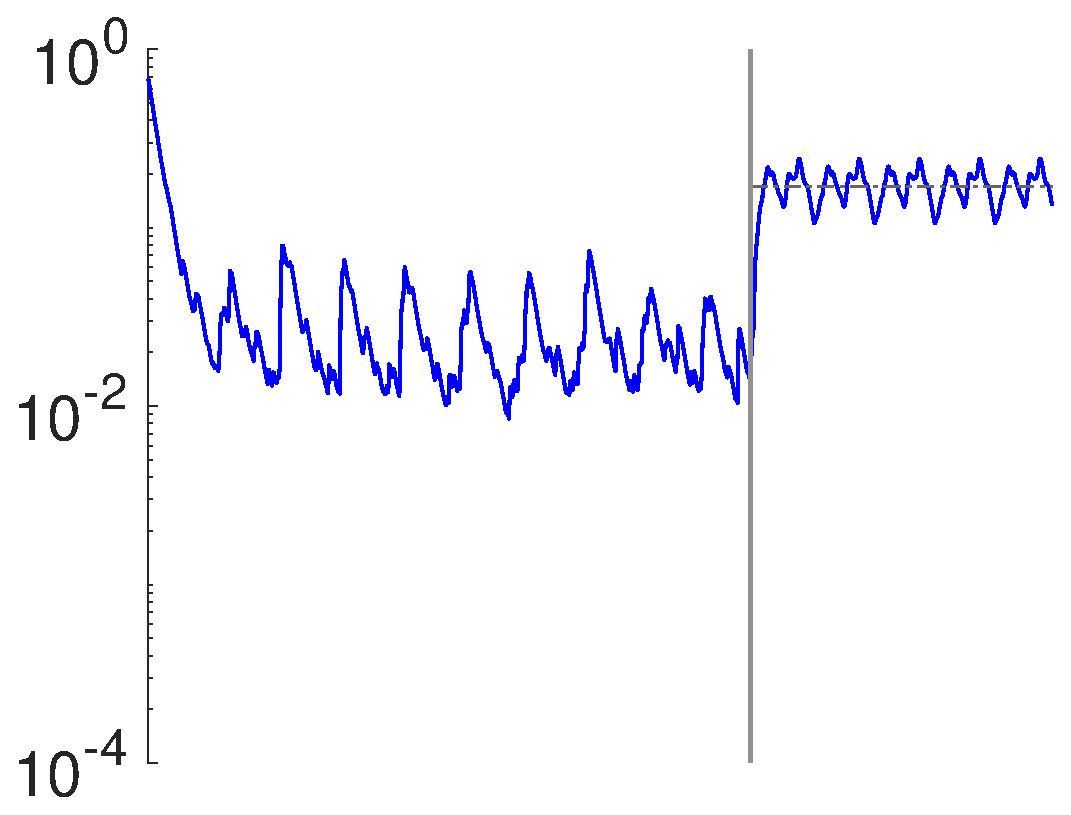
\includegraphics[height=0.12\linewidth,width=.45\linewidth]{Figures/Fig_T1/MATLAB/RHML_T1_MSE.eps}
        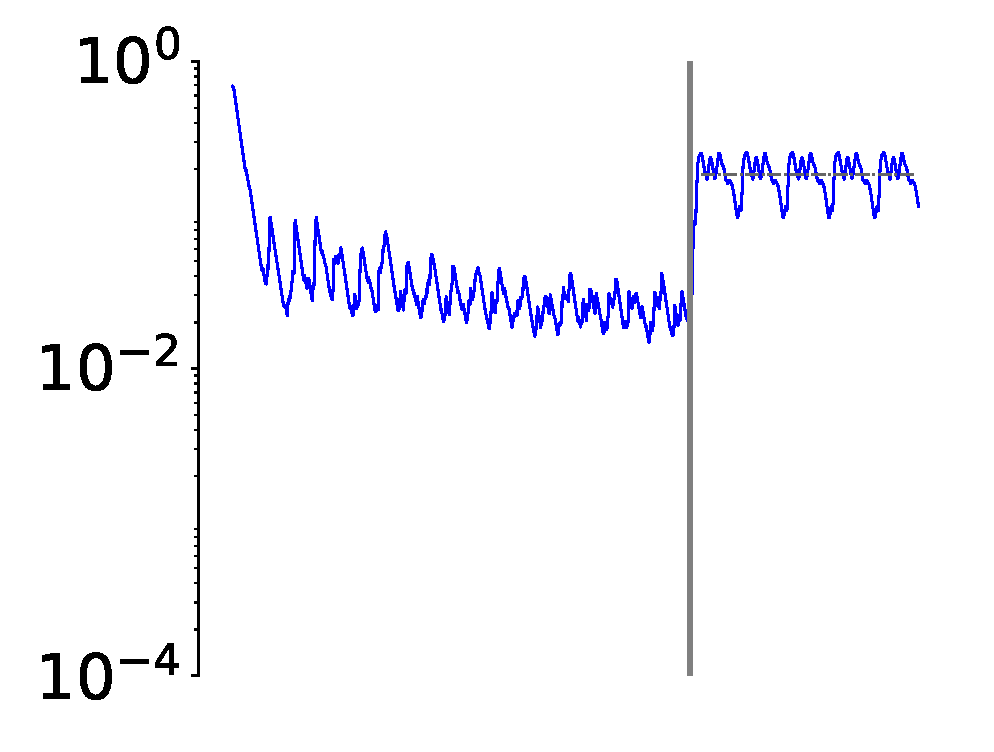
\includegraphics[height=0.12\linewidth,width=.45\linewidth]{Figures/Fig_T1/Python/RHML_T1_MSE.eps}
        
        \end{subfigure}
        
        
        \textbf{\rotatebox[origin=c]{90}{||W||}}\begin{subfigure}{\textwidth}
        \centering
        
        \includegraphics[trim=0cm 0cm 1cm 0cm, clip=true,height=0.12\linewidth,width=.45\linewidth]{Figures/Fig_T1/MATLAB/RHML_T1_W_norm.eps}
        \hspace{.3em}
        \includegraphics[trim=0cm 0cm 1cm 0cm, clip=true,height=0.12\linewidth,width=.45\linewidth]{Figures/Fig_T1/Python/RHML_T1_W_norm.eps}
        
        \end{subfigure}
        
    \caption{Results for Task 1 with the RMHL algorithm. The target time‐series is learned accurately during the training phase, though not maintained perfectly during the testing phase, as presented in \cite{pyle2019}.}
    \label{Fig:compTask1RMHL_MSE}
    \end{subfigure}
    
    \begin{subfigure}{\textwidth}
        \centering
        
        \textbf{\rotatebox[origin=c]{90}{SUPERTREX}}\begin{subfigure}{\textwidth}
        \centering
        
        
\includegraphics[trim=3cm 4cm 3cm 4cm, clip=true,height=.1\textheight]{Figures/Fig_T1/MATLAB/ST_T1_Trajectory.eps}
        \hspace{4em}
        
\includegraphics[height=.08\textheight]{Figures/Fig_T1/Orig/ST_T1_Trajectory.png}
        \hspace{4em}
        
\includegraphics[trim=6cm 4.5cm 6cm 4.5cm,clip=true,height=.1\textheight]{Figures/Fig_T1/Python/ST_T1_Trajectory.eps}
        
        \end{subfigure}
        
        \textbf{\rotatebox[origin=c]{90}{MSE}}\begin{subfigure}{\textwidth}
        \centering
        
        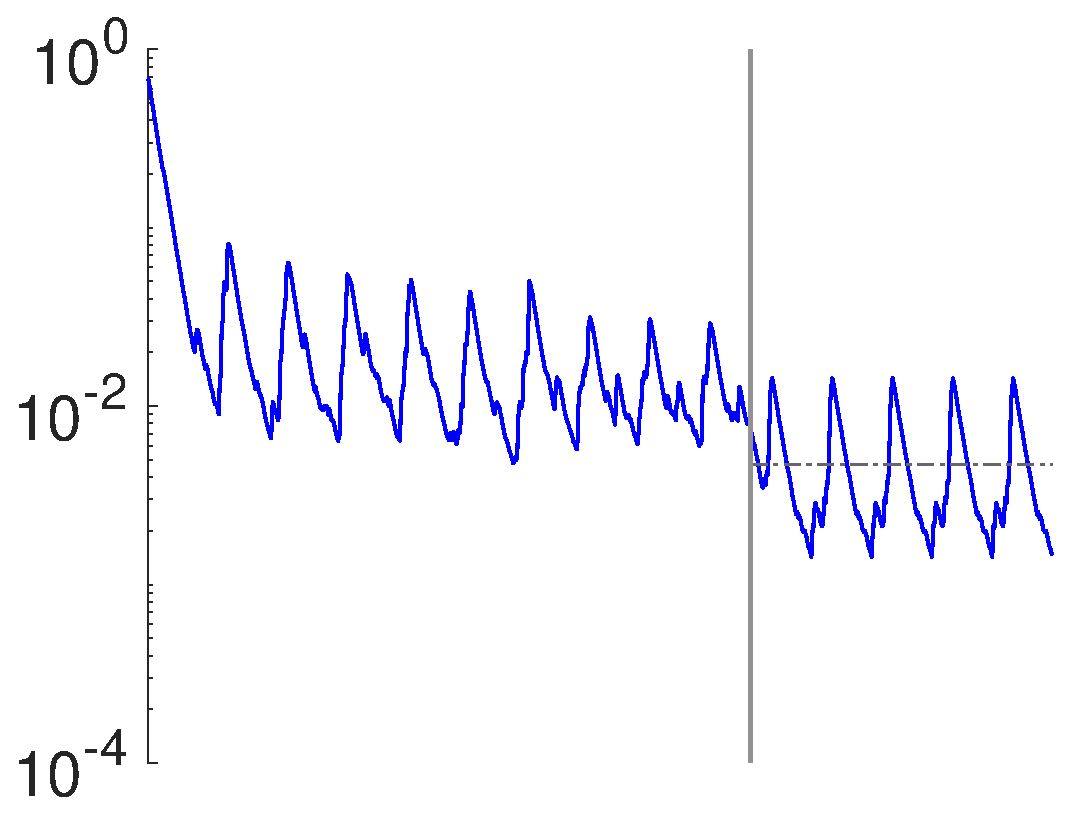
\includegraphics[height=0.12\linewidth,width=.45\linewidth]{Figures/Fig_T1/MATLAB/ST_T1_MSE.eps}
        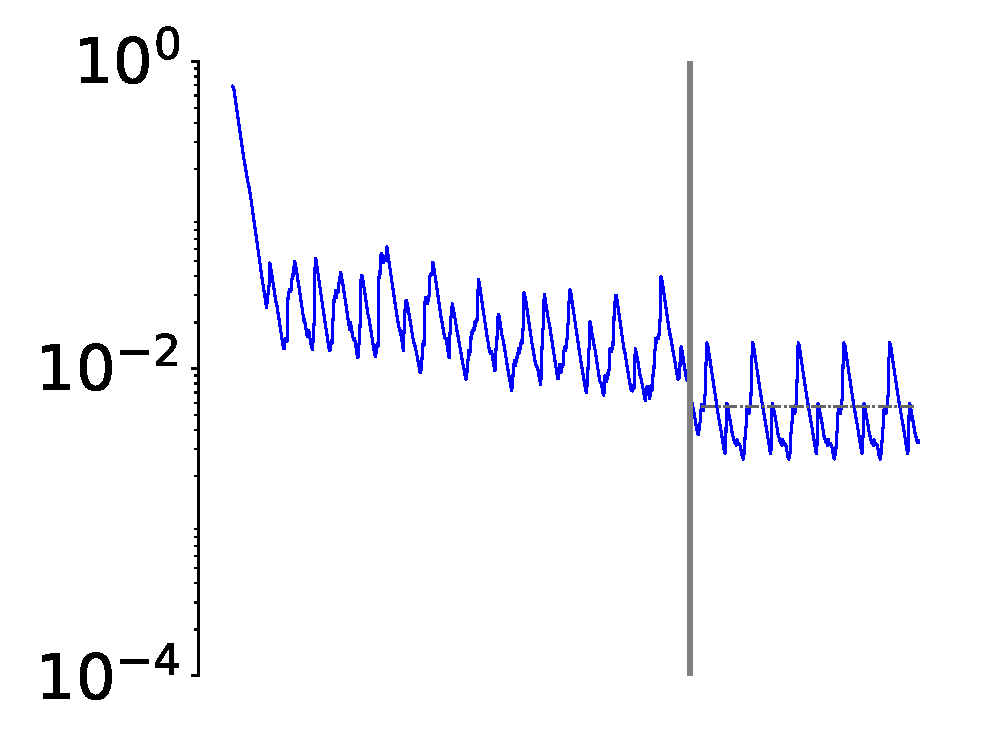
\includegraphics[height=0.12\linewidth,width=.45\linewidth]{Figures/Fig_T1/Python/ST_T1_MSE.eps}
        
        \end{subfigure}
        
        
        \textbf{\rotatebox[origin=c]{90}{||W||}}\begin{subfigure}{\textwidth}
        \centering
        
        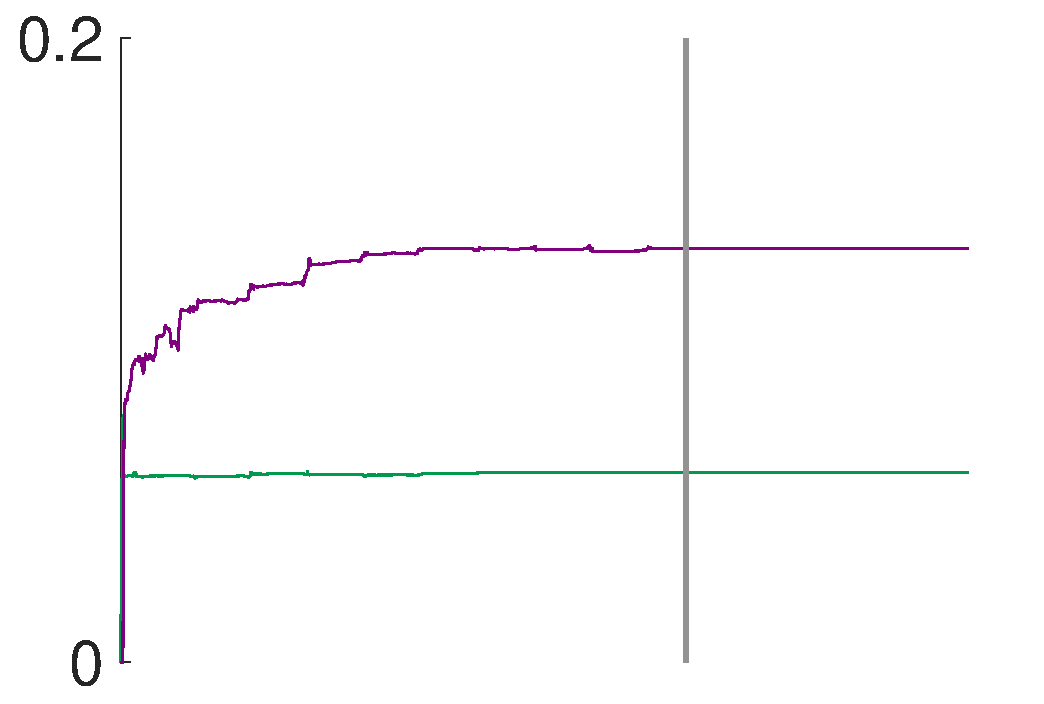
\includegraphics[trim=0cm 0cm 1cm 0cm, clip=true,height=0.12\linewidth,width=.45\linewidth]{Figures/Fig_T1/MATLAB/ST_T1_W_norm.eps}
        \hspace{.3em}
        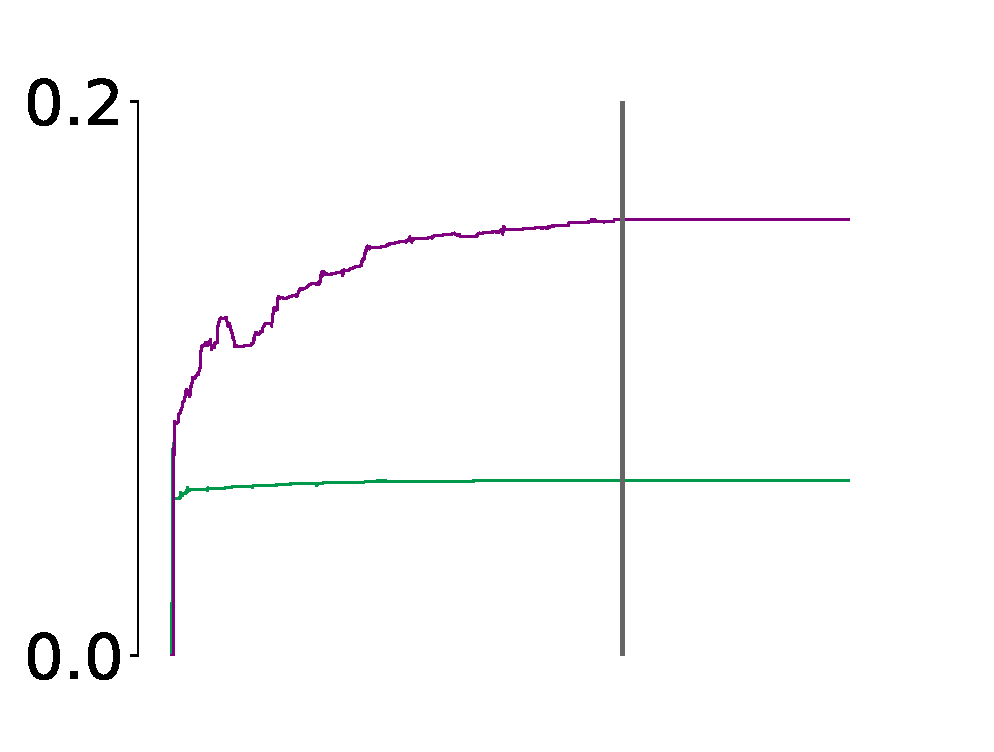
\includegraphics[trim=0cm 0cm 1cm 0cm, clip=true,height=0.12\linewidth,width=.45\linewidth]{Figures/Fig_T1/Python/ST_T1_W_norm.eps}
        
        \end{subfigure}


        
        
        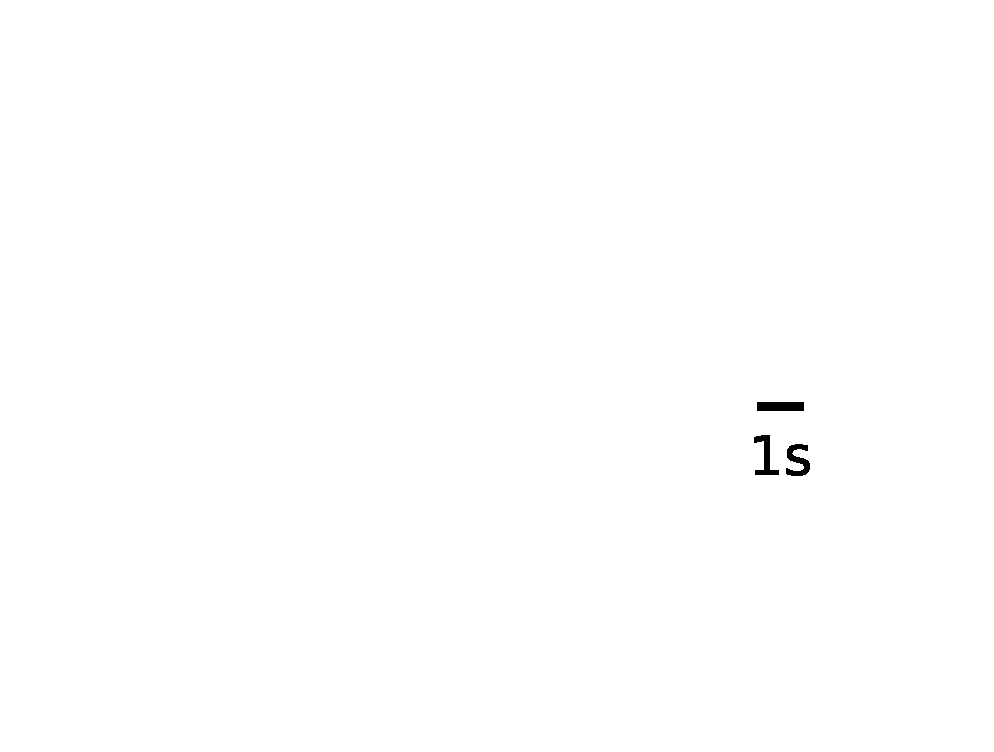
\includegraphics[trim=2cm 6cm 2cm 6cm, clip=true,height=0.05\linewidth,width=.4\linewidth]{Figures/Fig_T1/Python/ST_T1_Scale.eps}
        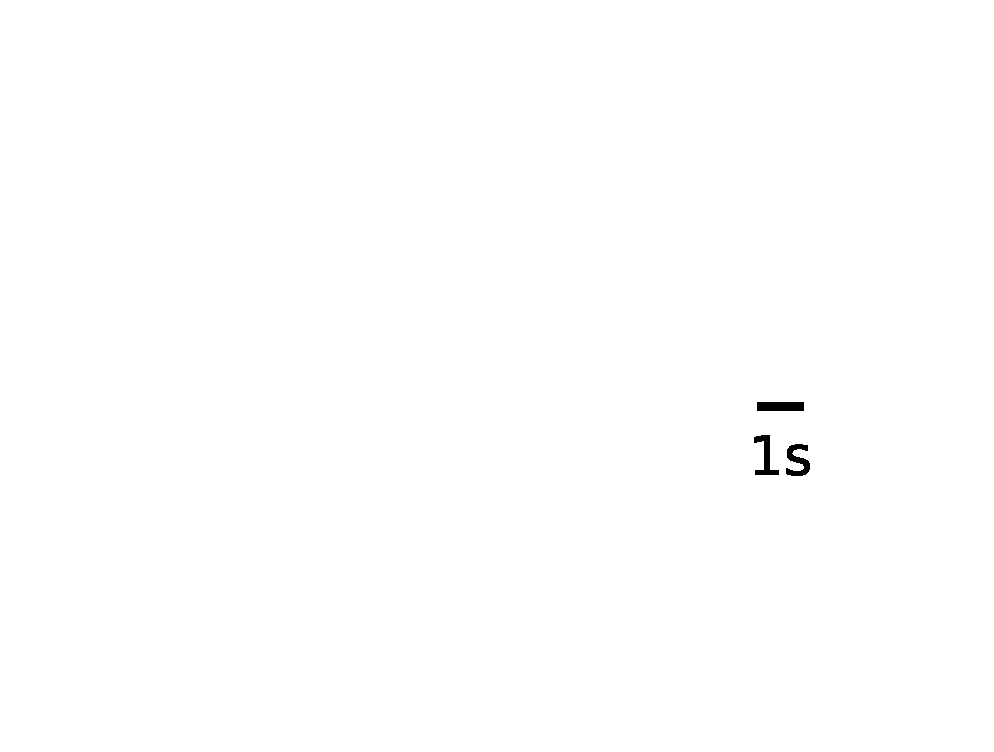
\includegraphics[trim=2cm 4cm 2cm 6cm, clip=true,height=0.05\linewidth,width=.45\linewidth]{Figures/Fig_T1/Python/ST_T1_Scale.eps}
        

    \caption{Results for Task 1 with the SUPERTREX algorithm. The target time‐series is learned accurately during the training phase, and is also maintained in a stable manner during testing phase, albeit not as well as FORCE, as presented in \cite{pyle2019}.}
    \label{Fig:compTask1ST_MSE}
    
    \end{subfigure}


\caption{Comparison of the performances of the MATLAB scripts (left column) and the Python adaptation (right column) with the results presented in the original article (center column), for the three learning algorithms on Task 1 \cite{pyle2019}. All simulations shown here use the MATLAB default (5489) as the seed for the random number generator. In each subfigure, the top row shows the target trajectory (red) with the trajectory generated by the model (blue) throughout the test phase. The second row shows the error metric (blue) over the simulation (x and y coordinates, in this case), using the log scale for the y axis. The bottom row shows the progression of the corresponding weight matrices (SUPERTREX: $W_1$ in purple; $W_2$, in green). The horizontal grey line, in the test phase, indicates the deviation metric.}
\label{Fig:Comparison_Task1_MSE}

\end{figure}




\subsection{Task 2}
Here, we compare the simulations of the original scripts and our Python adaptation for Task 2, using FORCE, RMHL and SUPERTREX, with the results presented in the article. Task 2 is designed to test the performance of these three algorithms when generating an unknown target from an indirect error signal. Using the paradigm of a pivoted multi-segmented arm, the objective of this task is to produce a time‐series by generating the angles between the arm segments. Motor output does not control the position of the end-effector of the arm, but instead controls the angles of the arm joints, which are non-linearly related to end-effector position.\\

The article claims that:
\begin{itemize}
\item the FORCE framework cannot be applied to this task, as FORCE requires the exact target to be provided as a supervisory error, which in this case would be the unknown target angles. Since, we do not have this information beforehand, and require the model to derive it, the FORCE framework is inapplicable to this task.  
\item under the RMHL framework, the target time-series is imitated well by the model during the training phase, however the weights do not converge, and hence, it is unable to maintain the time-series in a stable manner during the testing phase (Figure~\ref{Fig:compTask2RMHL}).
\item under the SUPERTREX framework, the target time-series is learned accurately and is also generated in a stable manner, with minor divergences, during testing phase, owing to the contribution of the pathway based on the FORCE algorithm (Figure~\ref{Fig:compTask2ST}).
\end{itemize}

We verify these observations with the MATLAB scripts provided by the authors as well as with our Python adaptation. To do so, we run the simulations with the default seed of MATLAB and re-simulate it with ten arbitrary seeds initialising the random number generator. We do not modify any task conditions or model hyper-parameters.  


We observe that:
\begin{itemize}
\item indeed, the FORCE framework is inapplicable to this task.  
\item under the RMHL framework, the target time-series is imitated well by the model during the training phase, however the weights do not converge, and hence, it is unable to maintain the time-series in a stable manner during the testing phase. The mean deviation over eleven simulations, for both the original scripts ($0.759\pm0.284$; n=11) and the Python adaptation ($0.814\pm0.288$; n=11) is higher than the threshold of 0.5 (Figure~\ref{Fig:compTask2RMHL}).
\item under the SUPERTREX framework, the target time-series is learned accurately and is also generated in a stable manner, with minor divergences, during testing phase, owing to the contribution of the pathway based on the FORCE algorithm. The mean deviation over eleven simulations, for both the original scripts ($0.011\pm0.003$; n=11) and the Python adaptation ($0.012\pm0.005$; n=11) is below the threshold of 0.5 and much lower than that with RMHL (Figure~\ref{Fig:compTask2ST}).
\end{itemize}

The MATLAB scripts provided by the authors and the Python adaptation are able to successfully closely reproduce the results presented for Task 2 in the paper, with the default seed as well as with the 10 arbitrary seeds (Figure~\ref{Fig:Comparison_Task2}; Table~\ref{Table:deviation_tasks},~\ref{Table:deviation_prop_tasks}).


\begin{figure}

    \centering
    \textbf{MATLAB}\hspace{8em}
    \textbf{Original}\hspace{8em}
    \textbf{Python}
    

    \begin{subfigure}{\textwidth}
        \centering
        
        \textbf{\rotatebox[origin=c]{90}{RMHL}}\begin{subfigure}{\textwidth}
        \centering
        
        \hspace{-3em}
        
\includegraphics[trim=3cm 0cm 3cm 4cm, clip=true,height=.25\linewidth]{Figures/Fig_T3/MATLAB/RMHL_T2_Seg2_Trajectory.eps}
        \hspace{2em}
        \includegraphics[trim=1cm 0cm 0cm 0cm, clip=true,height=.25\linewidth]{Figures/Fig_T3/Orig/RMHL_T2_Trajectory.png}
        \hspace{3em}
        
\includegraphics[trim=6cm 1.25cm 6cm 4.25cm, clip=true,height=.25\linewidth]{Figures/Fig_T3/Python/RMHL_T2_Seg2_Trajectory.eps}
        
        \end{subfigure}
         
        
        \textbf{\rotatebox[origin=c]{90}{$\theta_1$}}\begin{subfigure}{\textwidth}
        \centering
        
        \includegraphics[height=0.1\linewidth,width=.45\linewidth]{Figures/Fig_T3/MATLAB/RMHL_T2_Seg2_Theta0.eps}
        \includegraphics[trim=2cm 1cm 2cm 1cm, clip=true,height=0.1\linewidth,width=.45\linewidth]{Figures/Fig_T3/Python/RMHL_T2_Seg2_Theta0.eps}
        
        \end{subfigure}
         
        
        \textbf{\rotatebox[origin=c]{90}{$\theta_2$}}\begin{subfigure}{\textwidth}
        \centering
        
        \includegraphics[height=0.1\linewidth,width=.45\linewidth]{Figures/Fig_T3/MATLAB/RMHL_T2_Seg2_Theta1.eps}
        \includegraphics[trim=2cm 1cm 2cm 1cm, clip=true,height=0.1\linewidth,width=.45\linewidth]{Figures/Fig_T3/Python/RMHL_T2_Seg2_Theta1.eps}
        
        \end{subfigure}
         
        
        \textbf{\rotatebox[origin=c]{90}{MSE}}\begin{subfigure}{\textwidth}
        \centering
        
        \hspace{-2em}
        \includegraphics[height=0.15\linewidth,width=.45\linewidth]{Figures/Fig_T3/MATLAB/RMHL_T2_Seg2_MSE.eps}
        \hspace{.5em}
        \includegraphics[height=0.15\linewidth,width=.45\linewidth]{Figures/Fig_T3/Python/RMHL_T2_Seg2_MSE.eps}
        
        \end{subfigure}
        
    \caption{Results for Task 2 with the RMHL algorithm. The target time‐series is imitated well by the model during the training phase (not shown), however, it is unable to maintain the time-series in a stable manner during the testing phase, in both implementations, as presented in \cite{pyle2019}.}
    \label{Fig:compTask2RMHL}
    \end{subfigure}
    
    \begin{subfigure}{\textwidth}
        \centering
        
        \textbf{\rotatebox[origin=c]{90}{SUPERTREX}}\begin{subfigure}{\textwidth}
        \centering
        
        \includegraphics[trim=4cm 4cm 4cm 4.5cm, clip=true,height=.2\linewidth]{Figures/Fig_T3/MATLAB/ST_T2_Seg2_Trajectory.eps}
        \hspace{2em}
        \includegraphics[trim=1cm 0cm 0cm 0cm, clip=true,height=.2\linewidth]{Figures/Fig_T3/Orig/ST_T2_Trajectory.png}
        \hspace{0em}
        \includegraphics[trim=6cm 4.5cm 6cm 5cm, clip=true,height=.2\linewidth]{Figures/Fig_T3/Python/ST_T2_Seg2_Trajectory.eps}
        
        \end{subfigure}
        
        
        \textbf{\rotatebox[origin=c]{90}{$\theta_1$}}\begin{subfigure}{\textwidth}
        \centering
        
        \includegraphics[height=0.1\linewidth,width=.45\linewidth]{Figures/Fig_T3/MATLAB/ST_T2_Seg2_Theta0.eps}
        \includegraphics[trim=2cm 1cm 2cm 1cm, clip=true,height=0.1\linewidth,width=.45\linewidth]{Figures/Fig_T3/Python/ST_T2_Seg2_Theta0.eps}
        
        \end{subfigure}
        
        
        \textbf{\rotatebox[origin=c]{90}{$\theta_2$}}\begin{subfigure}{\textwidth}
        \centering
        
        \includegraphics[height=0.1\linewidth,width=.45\linewidth]{Figures/Fig_T3/MATLAB/ST_T2_Seg2_Theta1.eps}
        \includegraphics[trim=2cm 1cm 2cm 1cm, clip=true,height=0.1\linewidth,width=.45\linewidth]{Figures/Fig_T3/Python/ST_T2_Seg2_Theta1.eps}
        
        \end{subfigure}
         
        
        \textbf{\rotatebox[origin=c]{90}{MSE}}\begin{subfigure}{\textwidth}
        \centering
        
        \hspace{-2em}
        \includegraphics[height=0.15\linewidth,width=.45\linewidth]{Figures/Fig_T3/MATLAB/ST_T2_Seg2_MSE.eps}
        \hspace{.5em}
        \includegraphics[height=0.15\linewidth,width=.45\linewidth]{Figures/Fig_T3/Python/ST_T2_Seg2_MSE.eps}
        
        \end{subfigure}
        

        
        
        \includegraphics[trim=2cm 6cm 2cm 6cm, clip=true,height=0.05\linewidth,width=.4\linewidth]{Figures/Fig_T1/Python/ST_T1_Scale.eps}
        \includegraphics[trim=2cm 4cm 2cm 6cm, clip=true,height=0.05\linewidth,width=.45\linewidth]{Figures/Fig_T1/Python/ST_T1_Scale.eps}
        
        
    \caption{Results for Task 2 with the SUPERTREX algorithm. The target time‐series is learned accurately during the training phase, and is also maintained in a stable manner, during the testing phase, in both implementations, as presented in \cite{pyle2019}.}
    \label{Fig:compTask2ST}
    
    \end{subfigure}


\caption{Comparison of the performances of original scripts (left column) and Python adaptation (right column) with the results presented in the original article (center column), for the RMHL and SUPERTREX, on Task 2 \cite{pyle2019}. All simulations shown here use the MATLAB default (5489) as the seed for the random number generator. In each subfigure, the top row shows the target trajectory (red) with the trajectory generated by the algorithm (blue) throughout the test phase. The second row shows the time-series (blue) generated by the model (joint angles ($\theta_i$), in this case). The bottom row shows the distance from target metric (blue) over the simulation (x and y coordinates, in this case), using the log scale for the y axis. The horizontal grey line, in the test phase, indicates the deviation metric. The grey vertical line marks the separation of the training and testing phase.}
\label{Fig:Comparison_Task2}

\end{figure}


\subsection{Task 3}
Here, we compare the performance of the MATLAB scripts and our Python adaptation on Task 3, for the three algorithms, with the results presented in the article. Task 3 is an extension of Task 2, designed to test the constraint optimisation ability of these three algorithms when generating an unknown target from an indirect error signal. Using the paradigm of a pivoted multi-segmented arm, the objective of this task is to produce a time‐series by generating the angles between the arm segments, while also optimising the movement cost of each arm segment. Hence, the arm is required to traverse the butterfly, while carefully choosing the segment to rotate, in order to minimise the movement cost of its segments. Post the training phase, the readout weights are frozen and in the SUPERTREX model, the exploratory pathway is deactivated. \\

The article claims that:
\begin{itemize}
    \item FORCE can't be applied to this task, as explained for Task 2.
    \item under the RMHL framework, the target time-series is imitated well by the model during the training phase, however the weights do not converge, and hence, it poorly maintains the time-series during the testing phase (Figure~\ref{Fig:compTask3RMHL}).
    \item under the SUPERTREX framework, the performance is much better than RMHL. The target time-series is learned accurately and is also generated with minor divergences, during testing phase (Figure~\ref{Fig:compTask3ST}).
\end{itemize}

We verify these observations with the MATLAB scripts provided by the authors as well as with our Python adaptation. To do so, we run the simulations with the default seed of MATLAB and re‐simulate it with ten arbitrary seeds initialising the random number generator. 

We observe that:
\begin{itemize}
    \item indeed, the FORCE framework is inapplicable to this task, as claimed.  
    \item under the RMHL framework, the target time-series is imitated well by the model during the training phase, however the weights do not converge, and hence, it poorly maintains the time-series during the testing phase, as claimed. The mean deviation over eleven simulations, for both the original scripts ($0.850\pm0.313$; n=11) and the Python adaptation ($0.658\pm0.216$; n=11) is higher than the threshold of 0.5. All eleven simulations with different seeds did not generate the target output in a satisfactory manner (i.e. deviation $> 0.5$ for 11/11 seeds) (Figure~\ref{Fig:compTask3RMHL}).
    \item under the SUPERTREX framework, the performance is not much better than RMHL, contrary to the article's claim. The target time-series is not generated in a satisfactory manner, during the testing phase, for more than 50\% of the tested simulations (Original scripts: 6/11 and Python adaptation: 7/11). The mean deviation over eleven simulations, for both the original scripts ($0.881\pm0.224$; n=11) and the Python adaptation ($0.837\pm0.241$; n=11) is above the threshold of 0.5 and comparable with that of RMHL (Figure~\ref{Fig:compTask3ST}).
\end{itemize}

The original scripts and the Python adaptation are able to successfully reproduce the results presented in the paper with the default seed as well as with the 10 arbitrary seeds for the RMHL algorithm, but not for the SUPERTREX algorithm (Figure~\ref{Fig:Comparison_Task2}; Table~\ref{Table:deviation_tasks},~\ref{Table:deviation_prop_tasks}).







% \adjustbox{center}{
\begin{table}
\resizebox{\textwidth}{!}{%
% \adjustbox%{tabular=||c|c||c|c|c||c|c|c||c|c|c|,center}
\begin{tabular}{||p{1.8em}|c||c|c|c||c|c|c||c|c|c||}
 \hline
 \multicolumn{2}{||c||}{} & 
 \multicolumn{3}{|c||}{MATLAB} & \multicolumn{3}{|c||}{Python adaptation}  & \multicolumn{3}{|c||}{Python re-implementation}\\
 \hline
 Task & Model & Mean & Median & Std & Mean & Median & Std & Mean & Median & Std\\
 \hline
 \multirow{3}{4em}{   \#1  } & FORCE   & 
 0.003    & 0.002 &   0.002 & 
 0.004    & 0.003 &   0.003 & 
 0.003 &	0.002 &	0.003\\
 & RMHL  &
 0.168    & 0.165 &   0.038 & 
 0.182    & 0.182 &   0.046 & 
 0.201 &	0.203 &	0.053\\
 & ST  &
0.006    & 0.004 &   0.003 & 
 0.006    & 0.005 &   0.003 & 
0.004 &	0.003 &	0.003\\
 \hline
  \multirow{2}{4em}{ \#2} & RMHL   & 
0.759    & 0.740 &   0.284 & 
 0.814    & 0.799 &   0.288 & 
 0.697 &	0.681 &	0.263\\
 & ST &    
 0.011    & 0.010 &  0.003 & 
 0.012    & 0.011 &   0.005 & 
 0.010 &	0.009 &	0.004\\
 \hline
  \multirow{2}{4em}{\#3} & RMHL   & 
 0.850    & 0.794 &   0.313 & 
 0.658    & 0.647 &   0.216 & 
 0.849 &	0.794 &	0.360\\
 & ST &
 0.881     & 0.845 &   0.224 & 
 0.837    & 0.827 &   0.241 & 
0.140	& 0.116	& 0.071 \\
 \hline
  \multirow{2}{4em}{ \#2'} & RMHL   & 
0.846 &	0.807 &	0.299 & 
0.738 &	0.713 &	0.256 & 
0.839 &	0.794 &	0.310 \\
 & ST &    
0.016 &	0.015 &	0.007 & 
0.009 &	0.008 &	0.003 & 
0.067 &	0.062 &	0.035 \\
 \hline
\end{tabular}
% \end{adjustbox}
}
 \caption{Deviation metric showing the performance of the original MATLAB scripts, Python adaptation and Python re-implementation on different tasks. Each variant is simulated with the default seed (5489) and ten additional seeds. The mean, median and standard deviation of the deviation metric over these eleven simulations are tabulated here. Note that for task \#2', the SUPERTREX statistics have been computed using only 2 simulations, for the  original MATLAB scripts and Python adaptation. (ST: SUPERTREX; \#2': 3 segment variant of Task 2)}
  \label{Table:deviation_tasks}
\end{table}
% }


\begin{table}
\resizebox{\textwidth}{!}{%
\begin{tabular}{||p{2em}|c||c|c||c|c||c|c||}
 \hline
 \multicolumn{2}{||c||}{} & 
 \multicolumn{2}{|c||}{MATLAB} & \multicolumn{2}{|c||}{Python adaptation}  & \multicolumn{2}{|c||}{Python re-implementation}\\
 \hline
 Task & Model & Satisfactory & Total & Satisfactory & Total  & Satisfactory & Total  \\
 \hline
 \multirow{3}{4em}{   \#1  } & FORCE   & 
11	&   11 & 
11	&   11 & 
11	&   11\\
 & RMHL  &
11	&   11 & 
11	&   11 & 
11	&   11\\
 & ST  &
11	&   11 & 
11	&   11 & 
11	&   11\\
 \hline
  \multirow{2}{4em}{ \#2} & RMHL   & 
0	&   11 & 
0	&   11 & 
0	&   11\\
 & ST &    
11	&   11 & 
11	&   11 & 
11	&   11\\
 \hline
  \multirow{2}{4em}{\#3} & RMHL   & 
1	&   11 & 
2	&   11 & 
0	&   11\\
 & ST &
5   &	11 & 
4	&   11 & 
10	&   11 \\
 \hline
  \multirow{2}{4em}{ \#2'} & RMHL   & 
0	&   11 & 
1	&   11 & 
0	&   11 \\
 & ST &    
2	&   2 & 
2	&   2 & 
11	&   11 \\
 \hline
\end{tabular}
}
% \end{adjustbox}
 \caption{The proportion of model simulations categorised as having satisfactory performance. Each variant is simulated with the default seed (5489) and ten additional seeds. Number of satisfactory simulations refers to the number of simulations that were below the threshold (0.5) for the deviation metric. The total number of simulations refer to the number of simulations which successfully reached completion, without the weights growing exponentially.  (ST: SUPERTREX; 2': 3 segment variant of Task 2)}
  \label{Table:deviation_prop_tasks}
 \end{table}




\begin{figure}

    \centering
    \textbf{MATLAB}\hspace{8em}
    \textbf{Original}\hspace{8em}
    \textbf{Python}
    

    \begin{subfigure}{\textwidth}
        \centering
        
        \textbf{\rotatebox[origin=c]{90}{RMHL}}\begin{subfigure}{\textwidth}
        \centering
        
        \hspace{-1em}
        \includegraphics[trim=3cm 0.5cm 3cm 4cm, clip=true, height=.25\linewidth]{Figures/Fig_T4/MATLAB/RMHL_T3_Trajectory.eps}
        \hspace{3em}
        \includegraphics[trim=1cm 0cm 1cm 0cm, clip=true,scale=0.5,
        height=.25\linewidth]{Figures/Fig_T4/Orig/RMHL_T3_Trajectory.png}
        \hspace{3em}
        \includegraphics[trim=6cm 4.5cm 6cm 3cm, clip=true,  height=.25\linewidth]{Figures/Fig_T4/Python/RMHL_T3_Trajectory.eps}
        
        \end{subfigure}
         
        
        
    \caption{Results for Task 3 with the RMHL algorithm, using the default seed (5489) for the random number generator. The target trajectory is imitated well by the model during the training phase (not shown), however, it poorly maintains the time-series during the testing phase, in both implementations, as presented in \cite{pyle2019}.}
    \label{Fig:compTask3RMHL}
    \end{subfigure}
    
    \begin{subfigure}{\textwidth}
        \centering
        
        \textbf{\rotatebox[origin=c]{90}{SUPERTREX}}\begin{subfigure}{\textwidth}
        \centering
        
        \hspace{0em}
        \includegraphics[trim=4cm 4.25cm 4cm 3.5cm, clip=true, height=.2\linewidth]{Figures/Fig_T4/MATLAB/ST_T3_Trajectory.eps}
        \hspace{2em}
        \includegraphics[trim=0cm 0cm 1cm 0cm, clip=true, height=.15\linewidth]{Figures/Fig_T4/Orig/ST_T3_Trajectory.png}
        \hspace{-.25em}
        \includegraphics[trim=4cm 4.75cm 4cm 3.5cm, clip=true,  height=.2\linewidth]{Figures/Fig_T4/Python/ST_T3_Trajectory.eps}
        \hspace{-3em}
        
        \end{subfigure}
        
        
        \textbf{\rotatebox[origin=c]{90}{$\theta_1$}}\begin{subfigure}{\textwidth}
        \centering
        
        \includegraphics[height=0.1\linewidth,width=.45\linewidth]{Figures/Fig_T4/MATLAB/ST_T3_Theta0.eps}
        \includegraphics[trim=2cm 1cm 2cm 1cm, clip=true, height=0.1\linewidth,width=.45\linewidth]{Figures/Fig_T4/Python/ST_T3_Theta0.eps}
        
        \end{subfigure}
        
        
        \textbf{\rotatebox[origin=c]{90}{$\theta_2$}}\begin{subfigure}{\textwidth}
        \centering
        
        \includegraphics[height=0.1\linewidth,width=.45\linewidth]{Figures/Fig_T4/MATLAB/ST_T3_Theta1.eps}
        \includegraphics[trim=2cm 1cm 2cm 1cm, clip=true,height=0.1\linewidth,width=.45\linewidth]{Figures/Fig_T4/Python/ST_T3_Theta1.eps}
        
        \end{subfigure}
        
        
        \textbf{\rotatebox[origin=c]{90}{$\theta_3$}}\begin{subfigure}{\textwidth}
        \centering
        
        \includegraphics[height=0.1\linewidth,width=.45\linewidth]{Figures/Fig_T4/MATLAB/ST_T3_Theta2.eps}
        \includegraphics[trim=2cm 1cm 2cm 1cm, clip=true,height=0.1\linewidth,width=.45\linewidth]{Figures/Fig_T4/Python/ST_T3_Theta2.eps}
        
        \end{subfigure}
        
        
        \textbf{\rotatebox[origin=c]{90}{MSE}}\begin{subfigure}{\textwidth}
        \centering
        
        \hspace{-1.9em}
        \includegraphics[height=0.2\linewidth,width=.45\linewidth]{Figures/Fig_T4/MATLAB/ST_T3_MSE.eps}
        \hspace{.75em}
        \includegraphics[height=0.2\linewidth,width=.45\linewidth]{Figures/Fig_T4/Python/ST_T3_MSE.eps}
        
        \end{subfigure}
        
        
        
        \includegraphics[trim=2cm 6cm 2cm 6cm, clip=true,height=0.05\linewidth,width=.4\linewidth]{Figures/Fig_T1/Python/ST_T1_Scale.eps}
        \includegraphics[trim=2cm 4cm 2cm 6cm, clip=true,height=0.05\linewidth,width=.45\linewidth]{Figures/Fig_T1/Python/ST_T1_Scale.eps}
        

    \caption{Results for Task 3 with the SUPERTREX algorithm using the default seed (5489) for the random number generator. The target time‐series is learned accurately during the training phase, but is not maintained during the testing phase, in both implementations, in contrast to the results presented in \cite{pyle2019}.}
    \label{Fig:compTask3ST}
    
    \end{subfigure}
    
    \begin{subfigure}{\textwidth}
        \centering
        
        \textbf{\rotatebox[origin=c]{90}{SUPERTREX}}\begin{subfigure}{\textwidth}
        \centering
        
        \includegraphics[trim=4cm 4.25cm 4cm 4.75cm, clip=true, height=.2\linewidth]{Figures/Fig_T4/MATLAB/ST_T3_Trajectory_295728336.eps}
        \hspace{1em}
        \includegraphics[height=.2\linewidth]{Figures/Fig_T4/Orig/ST_T3_Trajectory.png}
        \hspace{1em}
        \includegraphics[trim=6.5cm 4.75cm 6.5cm 5cm, clip=true,  height=.2\linewidth]{Figures/Fig_T4/Python/ST_T3_Trajectory_5624282.eps}
        
        \end{subfigure}
        

    \caption{Results for Task 3 with the SUPERTREX algorithm using different implementations (MATLAB, left and Python adaptation, right) and different seeds (295728336, left and 5624282, right) for the random number generator. The target trajectory is learned accurately during the training phase, and is also maintained in a stable manner, with slight divergences (Deviation: 295728336: $0.215\pm0.073$; 5624282: $0.190\pm0.054$) , during the testing phase, in both implementations, similar to the results presented in \cite{pyle2019}.}
    \label{Fig:compTask3STrseeed2}
    
    \end{subfigure}

        
\caption{Comparison of the performances of original scripts (left column) and Python adaptation (right column) with the results presented in the original article (center column), for RMHL and SUPERTREX, on Task 3 \cite{pyle2019}. Each subfigure shows the target trajectory (red) with the trajectory generated by the algorithm (blue) throughout the test phase. In the second subfigure, the the middle rows show the time-series (blue) generated by the model (joint angles ($\theta_i$), in this case). The bottom row shows the distance from target metric (blue) over the simulation (x and y coordinates, in this case), using the log scale for the y axis.  The horizontal grey line, in the test phase, indicates the deviation metric. The grey vertical line marks the separation of the training and testing phase.}
\label{Fig:Comparison_Task3}

\end{figure}